%%%%%%%%%%%%%%%%%%%%%%%%%%%%%%%%%%%%%%%%%%%%%%%%%%%%%%%%%%%%%%%%%%%%%%%%%%%%%%%%
\chapter{Evaluation}
%%%%%%%%%%%%%%%%%%%%%%%%%%%%%%%%%%%%%%%%%%%%%%%%%%%%%%%%%%%%%%%%%%%%%%%%%%%%%%%%
\label{sec:evaluation}

\revision{In evaluating Landslide, we sought to answer two overall questions.

\begin{itemize}
	\item Is Landslide an effective use of time by a developer seeking to find and understand race conditions in their code? How can Landslide be improved to improve the time tradeoff?
	\item When testing kernel code with a systematic testing framework, what overall use patterns are most effective for getting meaningful results? How can future work employ such patterns to build more sophisticated systematic testing tools for kernels?
\end{itemize}

To answer these questions, we evaluated Landslide in two ways.}
First, we conducted a user study with students of 15-410 during the spring 2012 semester, to understand the ease and difficulty of Landslide's user interface process, to understand how to polish it into a more useful debugging tool.
Second, we did a case study of six bugs in two kernels, investigating them in-depth to understand how systematic testing might best be harnessed to find bugs without in advance knowing the decision set necessary to expose them.

\section{User Experience}
\label{sec:eval-studence}

To evaluate the experience of non-expert users working with Landslide, we met with 5 groups of students in 15-410 (9 students in total) during the final week of the kernel project in spring 2012, and had them use Landslide with their own kernels. \revision{Additionally, one former 15-410 Teaching Assistant (TA) participated in the study.}

In order to garner student interest in Landslide, the author gave a lecture in 15-410 on systematic exploration in general and on Landslide specifically during the second-to-last week of the kernel project.\footnote{
The lecture slides are available at \url{http://www.cs.cmu.edu/~410-s12/lectures/L30_Landslide.pdf}, and at \url{http://bblum.net/landslide-lecture.pdf}, and at \url{http://www.contrib.andrew.cmu.edu/~bblum/landslide-lecture.pdf}.}

We wished to measure which phases of using Landslide are most time-consuming, so we asked students \revision{in intervals between 30 and 60 minutes} to record the amount of time they had spent doing each phase:

\begin{enumerate}
	\item Annotating their kernel (Section~\ref{sec:using-annotations}).
	\item Implementing instrumentation within Landslide (Section~\ref{sec:using-student-c}).
	\item Fixing problems encountered getting Landslide to run, such as editing their kernel to meet Landslide's requirements and debugging incorrect instrumentation.
	\item Customising Landslide's search parameters such as decision points (Section~\ref{sec:using-customise}).
	\item Analysing the output from bugs that Landslide found.
\end{enumerate}

We also wanted descriptive feedback, to evaluate which specific parts of the process of using Landslide need improved. We asked students to write brief remarks whenever they recorded amounts of time spent, and also after they were finished to answer the following questions.

\begin{itemize}
	\item Were you able to get Landslide to work with your kernel (i.e., run through a minimal exploration tree completely)? If so, how long did it take, from sitting down to getting it to work? If not, did your kernel do something that was incompatible with Landslide, or were you unable to get the instrumentation right for some other reason?
	\item Did you find bugs while using Landslide, that you imagine would have been very hard to find otherwise? Did Landslide's output help you understand what caused them?
	\item Were you able to get Landslide to say ``you survived!'' with custom decision points? Did you think the set of decision points you used for this provide a strong guarantee about the absence of races?
	\item Describe your experience configuring the set of decision points. What was intuitive, obvious to do? Did you feel stuck at any point, not knowing where to go next?
	\item Was there anything you wanted to make Landslide do that it didn't support?
\end{itemize}

Finally, we briefly studied each bug that the students found: whether they were deterministic or race conditions, whether they were deep unsolved concurrency problems or simple oversights, and the complexity of the necessary fixes.

\revision{Of five student groups that we worked with during the user study, four groups completed the instrumentation process and got Landslide to explore at least a minimal decision tree. (A minimal decision tree is one resulting from decision points only on voluntary reschedules, which Landslide automatically identifies.)}

\subsection{Time Breakdown}

\newcommand\asdf[1]{\hspace{-0.05in}\footnotesize\bf{#1}\hspace{-0.05in}}
\revision{
\begin{table}[t]
	\begin{center}
	\small
	\begin{tabular}{|l||c|c|c|c|c|c||c|c|}
		\hline
		\multirow{2}{*}{\bf Group} & \multicolumn{6}{|c||}{\bf Minutes spent doing\dots} & \multicolumn{2}{|c|}{\bf Total time spent} \\
		\cline{2-9}
		& \asdf{annotating} & \asdf{config} & \asdf{student.c} & \asdf{fixing} & \asdf{customising} & \asdf{found races} & \asdf{required} & \asdf{refinement} \\
		\hline \hline
		% ntaha/jmchow
		\multirow{2}{*}{Group 1} & 35 & {\footnotesize \em N/A} & {\footnotesize \em N/A} & 5 & {\footnotesize \em N/A} & {\footnotesize \em N/A} & {\footnotesize \em N/A} & {\footnotesize \em N/A} \\
		\cline{2-9}
		& 5 & 30 & 10 & 100 & {\footnotesize \em N/A} & {\footnotesize \em N/A} & 145 & {\footnotesize \em N/A} \\
		\hline
		% echo/margaret
		\multirow{2}{*}{Group 2} & 20 & 30 & 10 & 80 & {\footnotesize \em N/A} & 10 & 140 & 10 \\
		\cline{2-9}
		& 15 & 45 & 30 & 60 & {\footnotesize \em N/A} & 30 & 150 & 30 \\
		\hline
		% tpassaro
		\multirow{2}{*}{Group 3} & 15 & 10 & 5 & 60 & 30 & 30 & 90 & 60 \\
		\cline{2-9}
		& 15 & 10 & 5 & 60 & 30 & 30 & 90 & 60 \\
		\hline
		% pjumde
		\multirow{2}{*}{Group 4} & 10 & 42 & 3 & 5 & 30 & {\footnotesize \em N/A} & 60 & 30 \\
		\cline{2-9}
		& 15 & 35 & {\footnotesize \em N/A} & 5 & 35 & {\footnotesize \em N/A} & {\footnotesize \em N/A} & 35 \\
		\hline
		% apodolsk
		Group 5 & 50 & 15 & {\footnotesize \em N/A} & 15 & {\footnotesize \em N/A} & {\footnotesize \em N/A} & {\footnotesize \em N/A} & {\footnotesize \em N/A} \\
		\hline
		Former TA & 40 & 20 & 3 & 95 & {\footnotesize \em N/A} & 30 & 158 & 30 \\
		\hline
		\hline
		{\bf Average } & {\bf 22 } & {\bf 26.33 } & {\bf 9.43 } & {\bf 48.5 } & {\bf 31.25 } & {\bf 26 } & {\bf 119 } & {\bf 36.43} \\
		\hline
	\end{tabular}
	\end{center}
	\caption{Self-reported times spent by users on each phase while using Landslide. ``N/A'' indicates a student reported spending no time on a particular phase. ``Required'' indicates the sum of the times from the first four phases; ``refinement'' inducates the sum from the last two phases.
	``N/A'' indicates that a user did not report spending any time on a phase; the ``required'' field is ``N/A'' if any of its represented phases are, and ``N/A'' fields are not reflected in the averages.}
	\label{fig:student-times}
\end{table}

While the students were using Landslide, we asked them at intervals from 30 to 60 minutes to record how much time they had spent on each phase of instrumenting and using Landslide.

\begin{itemize}
	\item {\bf Required instrumentation.} These phases represent work necessary to getting Landslide to work with a kernel at all.
	\begin{itemize}
		\item {\bf Annotating the kernel.} In this phase, the student modifies their kernel to use the provided annotations (Section~\ref{sec:using-annotations}).
		\item {\bf Writing the configuration file.} In this phase, the student fills out certain information about their kernel in \texttt{config.landslide} (Section~\ref{sec:using-config-landslide}).
		\item {\bf Instrumenting within Landslide.} In this phase, the student implements the two instrumentation functions in \texttt{student.c} (Section~\ref{sec:using-student-c}).
		\item {\bf Fixing instrumentation problems/crashing.} In this phase, the user repairs problems that arose due to incorrect instrumentation (or bugs in Landslide itself, in some cases).
	\end{itemize}
	\item {\bf Extra refinement.} These phases represent additional work to be done after successfully exploring a minimal decision tree. When such minimal exploration finds no bugs, such additional work is necessary to provide meaningful results.
	\begin{itemize}
		\item {\bf Customising decision points.} In this phase, the user configures Landslide to use decision sets more refined than the minimal one, in search of hard-to-find bugs (Section~\ref{sec:using-customise}).
		\item {\bf Investigating found race conditions.} In this phase, the user attempts to understand and fix bugs that Landslide found and reported.
	\end{itemize}
\end{itemize}

\begin{wrapfigure}{r}{0.4\textwidth}
	\center
	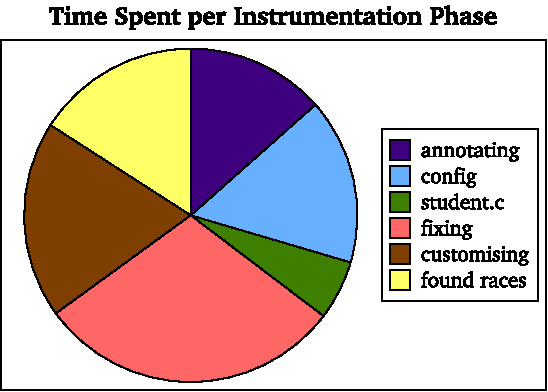
\includegraphics[width=0.4\textwidth]{graphs/studence-pie.pdf}
	\caption{Average time breakdown for each phase of instrumenting a kernel with Landslide, based on student self-reported times.}
	\label{fig:student-pie}
\end{wrapfigure}

Table~\ref{fig:student-times} presents the time breakdown among phases that students experienced while using Landslide, visualised in Figure~\ref{fig:student-pie}. On average, students spent two hours getting Landslide to work with their kernels, and slightly more than half an hour customising the search and/or studying found bugs on top of that.

We consider the absolute values of these numbers largely artifacts of the user interface's quality (i.e., they could be improved with extra interface polishing, though they also currently present an upper bound). The relative values among phases, however, serve to give a notion of which phases were most difficult.

We do not think it useful to consider these times amortised over how many bugs were found for each group, because in general we do not know whether each group would have found more bugs with marginal extra effort, having already paid the initial cost of instrumenting. (The vanish/vanish bug we describe finding ourselves in Section~\ref{sec:eval-victory-races} serves as an example of this perennial possibility.)
Instead, we claim that the fact that Landslide found bugs for all groups who completed the required instrumentation proves its baseline effectivness as a debugging tool, and we note that the time tradeoff will become more worthwhile the more the user interface improves.
}

\subsection{Descriptive Feedback}
\label{sec:eval-feedback}

The students provided specific remarks which fell into two categories: issues with Landslide's user interface, and needing to change something in one's kernel to make it work with Landslide.

\subsubsection{User Interface Feedback}

For Landslide to be appealing as a debugging tool, we should improve the user interface (or the infrastructure, in some cases) to address the following issues.

\begin{itemize}
	\item {\bf Difficulty of debugging incorrect instrumentation.} When the user-provided annotations/instrumentation are incorrect, Landslide's error messages are difficult to understand, and often don't point to the real problem.
	\item {\bf Interpreting debugging output.} Some students reported the decision trace representation could be better. One student reported the output was easy to follow by ``tracing the life of the buggy thread'', which is an insight into the learning process we should capitalise on.
	\item {\bf Ease of configuring decision sets.} Most students seemed to find the process of adding more decision points intuitive. One reported, ``quick and effective at detecting basic bugs/races.'' \revision{While this interface could always be improved, of all the parts of the user experience, this process seems to need it least.}
	\item {\bf General feature wishlist.} The following features, of varying difficulty to implement, would have improved user experience overall.
		\begin{itemize}
			\item Being able to continue exploration after interrupting Simics to work with the debug prompt, instead of having to start over.
			\item Support for multiprocessor kernels.
			\item Cutting down overall simulation time.
		\end{itemize}
\end{itemize}

\subsubsection{Technical Feedback}

Students also described compatibility issues they faced between their kernels and Landslide, which required them to make certain changes to their kernels.

\begin{itemize}
	\item {\bf Special-case context switch behaviour.} One kernel had a special context-switcher for the case when a thread was vanishing, which had to be special-cased in the instrumentation.
		Some kernels had different context switch designs for just-forked threads (as discussed in the ``Thread Creation'' bullet in Section~\ref{sec:challenges-design}), and Landslide's code had to be modified during the study to support different designs.
	\item {\bf Unexpected compiler optimisations.} Listing scheduler functions in \texttt{config.landslide} could be confusing if the compiler inlined them.
	\item {\bf Driver thread interfering with test lifecycle tracking.} One kernel (Pathos, the 15-410 reference kernel) had to be modified to ensure the keyboard thread ran once before the test started, which was not mandated by the kernel design. (If the thread didn't run, it would conflict with the population-tracking described in Section~\ref{sec:components-test}, and Landslide would not be able to detect when the test was over.)
	\item {\bf Kernel behaviour requirement violations.}
		The majority of groups needed to change their scheduling around the idle thread in order to meet the requirement that the kernel never run idle when progress could otherwise be made (Sections~\ref{sec:challenges-design} and \ref{sec:using-requirements-sched}).
		Also, one kernel had to have its custom memory allocator disabled, because Landslide only supports LMM, the allocator that 15-410 provides.

		\revision{The idle requirement is an inherent part of Landslide's model, whereas the dynamic allocator requirement could be replaced with a richer set of optional annotations.}
\end{itemize}

Additionally, two enterprising users found ways to avoid implementing the functions in \texttt{student.c} (Section~\ref{sec:using-student-c}). It is worth considering integrating these approaches into the recommended approach to eliminate the need for \texttt{student.c} entirely.
\begin{itemize}
	\item One student bypassed the \texttt{kern\_ready\_for\_timer\_interrupt} annotation by disabling their scheduler's preemption-disabling mechanism and replacing it with explicit disabling of interrupts. \revision{This caused the kernel to context switch every timer interrupt, so Landslide did not need to be aware of extra conditions that would cause the scheduler to ignore timer ticks.}
	\item The former TA was able to avoid the \texttt{kern\_current\_extra\_runnable} annotation by using the \texttt{on\_rq} and \texttt{off\_rq} annotations (Section~\ref{sec:using-annotations}) to express the ``abstract set of runnable threads'' (which included the currently-running thread, even though the runqueue didn't) instead of the literal runqueue itself. \revision{We did not advertise this method because we suspected students might make more mistakes instrumenting this way, but it might be worth advocating anyway for the sake of making the interface simpler.}
\end{itemize}

\subsection{Landslide Victories}
\label{sec:eval-victory}

Of the four groups that completed the required instrumentation, two found race conditions in their kernel. Additionally, Landslide helped all four groups find deterministic bugs: three groups had previously unknown problems with running the idle thread inappropriately, and the other group had a simple use-after-free.

We list how much progress each group made, and whether or not they found any bugs.

\begin{enumerate}
	\item % ntaha/jmchow
		Group 1 got Landslide to explore a minimal decision tree, and also explored \texttt{double\_wait} and \texttt{vanish\_vanish} with several combinations of different decision points around \texttt{mutex\_lock} and \texttt{mutex\_unlock}. They found one race and a problem with idle.
		After fixing these bugs, they were able to completely explore both test cases with decision points on both \texttt{mutex\_lock} and \texttt{mutex\_unlock}, which we consider a strong negative result (i.e., no bug found in those two test cases with fine-grained interleavings).
	\item % margaret/echo
		Group 2 got Landslide to explore a minimal decision tree. They did not configure any extra decision points. They found a problem with idle, and after fixing it, found a vanish-related race condition in the fix. They also found a bug in an assertion which they had added during the process, but that bug was deterministic, so we consider this part of the ``fixing incorrect instrumentation'' process.
	\item % tpassaro/?
		Group 3 got Landslide to explore a minimal decision tree, and also configured extra decision points for \texttt{vanish\_vanish}. They found only a deterministic use-after-free bug.
	\item % pjumde/?
		Group 4 got Landslide to explore a minimal decision tree. They found only a problem with idle.
	\item % apodolsk
		Group 5 did not invest enough time to get Landslide to explore a minimal decision tree.
\end{enumerate}

\subsubsection{Race Conditions Found}
\label{sec:eval-victory-races}

Two groups found race conditions using Landslide. We describe them here.

\begin{itemize}
	\item {\bf Too many waiters allowed.} Using the \texttt{double\_wait} test case, Group 1 found a bug in which more threads invoking \texttt{wait} would be allowed to block than the number of child processes that could ever be reaped, and some of the waiters would end up blocking forever. The fix for this was two lines of code. \revision{The group claimed it could have been found with an ``in-depth'' code review, though we claim Landslide's contribution here was still non-trivial, because (as exhibited here) such bugs exist anyway for lack of sufficient review.}
	\item {\bf Accidental return to a vanished thread.} Group 2 had a problem with the scheduler running idle when it was not supposed to; when they fixed it, however, their implementation would return to a thread that had already vanished in the case when no thread was left to run. It is unclear if this race would have been exposed without Landslide. Fixing it required adding an extra condition to the code that checked whether the kernel should idle.
\end{itemize}

We also note that, though Group 2 stopped using Landslide after getting it to explore the minimal decision tree, if they had configured decision points around \texttt{mutex\_lock} (which was the recommended next step in the process), they would have found a subtle race in the reparenting section of their \texttt{vanish} code using the \texttt{vanish\_vanish} test. We verified this by having an ex-TA re-instrument their kernel and add the decision points: from the time of exploring a minimal decision tree to finding the bug with the new decision set took half an hour of work, and fully understanding the nature of the bug took an hour on top of that.

This bug is similar to the LudicrOS vanish/vanish bug studied in Section~\ref{sec:eval-casestudy}, and would have required a complicated redesign of the \texttt{vanish} implementation to fix.

We consider this a mixed blessing: Landslide was capable of finding a deep concurrency bug in a student kernel, but the instrumentation process was expensive enough that they were not motivated to continue working, and stopped just short. We believe that improving Landslide's interface (Section~\ref{sec:future-interface}) will improve the success rate in such cases.

\subsubsection{Deterministic Bugs Found}

We also claim that Landslide is useful in its ability to find certain types of non-concurrency-related bugs. Though its primary purpose is to find race conditions, we found that it caught two main types of bugs that the students were previously unaware their kernels had.

\begin{itemize}
	\item {\bf Inappropriate idling.} Two groups had errors in their keyboard handling code, where when a newline was received when the kernel was idle, a thread blocked on \texttt{readline} would be added to the runqueue and but not switched directly to, so the kernel would continue idling even though there was useful work to do. Another group left idle on the scheduler runqueue, and had no special-case code to skip over it, so would interleave idle arbitrarily with other threads. We consider both of these performance problems.
	\item {\bf Deterministic use-after-free.} One group had a deterministic use-after-free bug in their \texttt{wait} implementation, in which they freed something and immediately dereferenced it. This hadn't presented a problem because the block was never reallocated during the critical window, which would have taken a complicated and fine-grained interleaving, but Landslide's heap checker detected the use-after-free immediately, without the need for any interleaving.
\end{itemize}

%%%%%%%%%%%%%%%%%%%%%%%%%%%%%%%%%%%%%%%%%%%%%%%%%%%%%%%%%%%%%%%%%%%%%%%%%%%%%%%%
\section{Bug Case Studies}
\label{sec:eval-casestudy}

While building Landslide, we worked primarily with two kernels: one, the kernel the author wrote as a student in 15-410 (Fall 2008), and another, a kernel the author graded as a TA for 15-410 (Fall 2011). We refer to the first kernel as ``POBBLES'' and to the second, with permission, as ``LudicrOS''.

With Landslide, we found four bugs in POBBLES and two bugs in LudicrOS, and investigated them more deeply.

\subsection{Bug Descriptions}

Here we describe each of the six bugs that we used as case studies. We rate their complexity and the estimated ease of fixing them.

\subsubsection{POBBLES vanish/vanish (a)}

We introduced this bug into POBBLES's vanish implementation. When a parent and child invoke vanish concurrently, the parent needs to modify the child's parent pointer to reparent it to the init process, and the child needs to read its parent pointer to signal to its parent that it can be reaped.

In version (a) of this bug, we introduce a mutex for each process's parent pointer.
\revision{While holding the lock around all related process structure accesses prevents data races, the circular nature of the lock acquisitions between parent and child results in deadlock.}

This bug is exposed with the \texttt{vanish\_vanish} test case. It requires a very specific interleaving sequence to uncover.
The fix is nontrivial, because the circular data structure access still needs to happen, but be protected in a way that doesn't involve circular wait.
Vanish races are notorious among 15-410 course staff as being difficult to find with the naked eye, and also difficult to figure out how to fix.

\subsubsection{POBBLES vanish/vanish (b)}

We also introduced this bug into POBBLES's vanish. Version (b) is similar to version (a), except we removed the parent pointer mutex entirely. This results in a data race around the parent pointer, in which the child can end up accessing the wrong parent either before or after it is actually moved to init's child-list.

This bug is exposed with the \texttt{vanish\_vanish} test case. The complexity and difficulty of fixing are the same as in version (a).

\subsubsection{POBBLES wait/wait}

Finding this bug was somewhat of a surprise. When two threads in the same process wait for a child to exit, they both block on the same condition variable, and one of them has a pointer to the other in its \texttt{cond\_queue\_next} pointer. However, when awakened, the condition variable code did not clear the value of this pointer. Fortunately, an assert statement in the thread destruction code caught that the pointer was non-\texttt{NULL} when it should have been \texttt{NULL}, and the kernel panicked.

Even with this assert, extremely mysterious behaviour could have arisen in other use cases, such as during stress testing: if the awakened thread had gone to sleep on another condition variable, its \texttt{cond\_queue\_next} pointer could point to a thread asleep on a different condition variable, in which case a broadcast on the new condition variable would cause a spurious wakeup of the second thread. Worse yet, if the second thread had also been awoken, and thence exited, a broadcast would result in scheduler data structure corruption.

This bug is exposed with the \texttt{double\_wait} test case.
The complexity of this bug is moderate, since it requires both waiting threads to block before the child process exits.
The fix is simple; in two places in the condition variable code a pointer needed to be set to \texttt{NULL}.

We note that the author never knew of its existence between submitting the kernel as a student three years ago and uncovering it before the user study three weeks ago, and it was not spotted by the TA who graded it.\footnote{
We would also note that this bug was never uncovered by any stress test, but the \texttt{double\_wait} test case was not distributed as part of the 15-410 test suite, and it was necessary to generate the right sequence of system calls.}

\subsubsection{POBBLES thread\_fork/wait}
\label{sec:eval-thread-fork}

This bug was presented in the lecture, and exhibited as a decision tree in Figure~\ref{fig:threadfork} and as a trace in Figure~\ref{fig:found_a_bug} and as source code in Figure~\ref{fig:tell-landslide}. When a new thread is forked and made runnable, and the forking thread subsequently dereferences its TID to use as a return value, it's possible for the dereference to be a use-after-free. This could result in a garbage value being returned.

This bug is exposed with the \texttt{double\_thread\_fork} test case. The complexity is relatively simple,\footnote{
Many userspace thread libraries forcibly serialise invocations of \texttt{thread\_fork} and \texttt{vanish} with their own synchronisation barriers, so the kernel bug may never be noticed when using such libraries (this caused the author some trouble).}
and the fix is only two lines long; the dereference should simply occur before making the child thread runnable.

Nevertheless, this bug was present in the author's student kernel and was not noticed by the TA who graded it.

\subsubsection{LudicrOS vanish/vanish}
\label{sec:eval-ludicros-vanish}

This bug was found by the author when grading this kernel. It took roughly an hour of manual inspection and hard thinking to ascertain the bug's nature, from the time when the author first suspected a bug might be present.

The parent pointer problem is the same as in the POBBLES vanish/vanish bugs, except the locking pattern is slightly different. When the parent reparents children, it drops its own mutex while it changes the parent pointer using the child's parent pointer mutex, which happens before the parent moves the child to init's child-list.

Many problems can arise from this error. The one Landslide discovered was as follows: During this gap, the child can take its own parent pointer mutex (after the pointer was changed to init), and attempt to move itself from init's ``live child-list'' to the ``dead child-list'' before the parent moved the child to init's child-list at all. This results in the child instead moving the {\em shell process} off of init's ``live child-list''. Init gets signalled, reaps the reparented child, does \texttt{wait} again (expecting the shell to be alive), which fails. This results in init infinitely looping around failing calls to \texttt{wait}. To catch this bug \revision{immediately, rather than relying on infinite loop detection,} we added an assert statement in the \texttt{wait} failure case that the current thread was not init (because init should always have children to reap or wait for), which Landslide then caused to trip.

This was the most complicated bug we studied. The fix would be nontrivial, like in POBBLES vanish/vanish.

\subsubsection{LudicrOS yield/vanish}

This bug was also found during grading, and took substantially less time to verify by hand than the previous bug. When a thread does \texttt{yield} to a specific other TID, the other thread's thread control block (TCB) is not protected \revision{after being returned from the look-up function}. If that thread exits during that time, a use-after-free (and worse, a completely invalid schedule to a nonexistent thread) results.

This bug is moderately complicated, requiring a preemption during that specific window of the first thread's execution during which the second thread must exit entirely and have its TCB freed. The fix is moderately complicated \revision{as well; since simply reordering lines of code won't offer the necessary protection.}

\subsection{Performance}
\label{sec:eval-numbers}

Table~\ref{fig:numbers} shows the time it takes to find each of these bugs using Landslide, configured with several different sets of decision points.
\revision{Figure~\ref{fig:number-graph} compares the total exploration time among each different decision set for the trials that did find bugs.}

\newcommand\bugnum[2]{\textcolor{BrickRed}{{\bf #1} {\scriptsize \em (#2)}}}
\newcommand\nobugnum[2]{\textcolor{Blue}{[{\em #1 {\scriptsize (#2)}}]}}

\begin{table}[t!]
	\begin{center}
	\small
	\begin{tabular}{|l||c|c|c|c|}
		\hline
		\multirow{2}{*}{\bf Kernel and test case} & \multicolumn{4}{c|}{\bf Decision points used} \\ % & \multirow{2}{*}{\bf Stress test} \\
		\cline{2-5}
		& {\bf default} & {\bf lock} & {\bf unlock} & {\bf both} \\
		\hline\hline
		POBBLES vanish/vanish (a) & \nobugnum{31.8}{0.6} & \bugnum{57.1}{1.7} & $\infty$ & $\infty$ \\
		\hline
		POBBLES vanish/vanish (b) & \nobugnum{32.0}{0.4} & \bugnum{51.5}{2.1} & \nobugnum{8057.9}{336.9} & $\infty$ \\
		\hline
		POBBLES wait/wait & \bugnum{23.3}{0.7} & \bugnum{27.9}{0.8} & \bugnum{27.9}{2.1} & \bugnum{41.6}{1.4} \\
		\hline
		POBBLES thread\_fork/vanish & \bugnum{22.0}{0.6} & \bugnum{37.4}{1.1} & \bugnum{27.6}{0.5} & \bugnum{72.0}{2.6} \\
		\hline
		LudicrOS vanish/vanish & \nobugnum{13.2}{0.2} & \bugnum{13.7}{0.7} & \bugnum{34.6}{1.1} & \bugnum{17.1}{0.3} \\
		\hline
		LudicrOS yield/vanish & \nobugnum{12.3}{0.3} & \bugnum{11.4}{0.4} & \nobugnum{27.4}{0.8} & \bugnum{11.7}{0.4} \\
		\hline
	\end{tabular}
	\end{center}
	\caption{Comparison of time taken (in seconds) to find bugs using Landslide with various decision sets:
	the default set, consisting only of voluntary reschedules (Section~\ref{sec:components-arbiter}); and using custom decision points in addition to the default set: calls to \texttt{mutex\_lock}, calls to \texttt{mutex\_unlock}, and both.
	All numbers represent the average from 5 trials, with the standard deviations given in parentheses. \\
	Key: \bugnum{seconds}{\footnotesize stddev} indicates bug found; \nobugnum{seconds}{\footnotesize stddev} indicates whole tree explored with no bug.
	``$\infty$'' indicates that Landslide's search did not finish (after 8 hours).
	}
	\label{fig:numbers}
\end{table}
\revision{
\begin{figure}[h]
	\center
	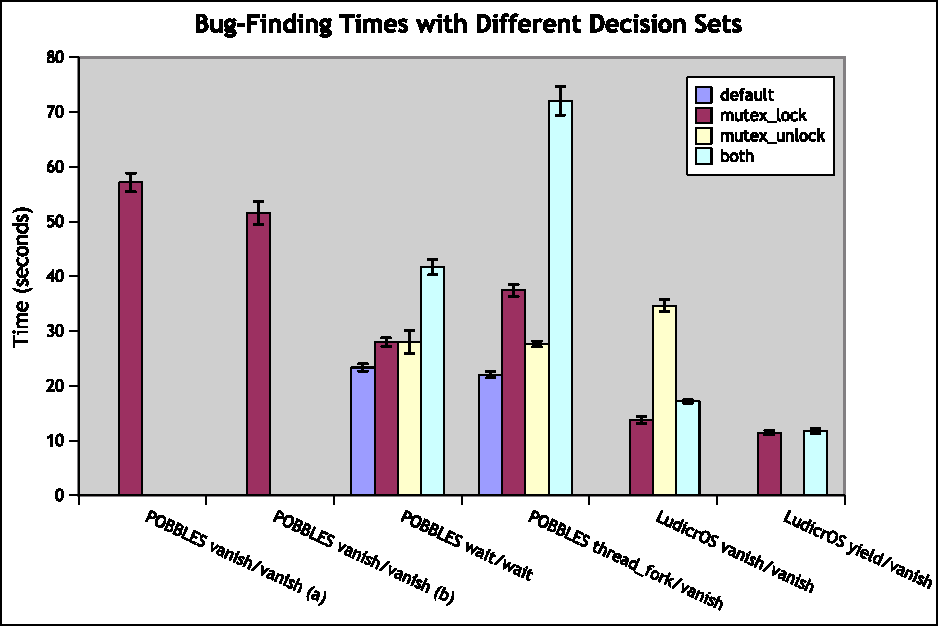
\includegraphics[width=0.8\textwidth]{graphs/decisions.pdf}
	\caption{Bar graph visualisation of the exploration time in trials that did find bugs. The decision trees that did not expose bugs and the ones that timed out are not shown.}
	\label{fig:number-graph}
\end{figure}
}

The experimental set-up is as follows:

\begin{itemize}
	\item All Landslide trial times include the Simics start-up and kernel boot-up time (time between issuing the command and the test case beginning to run), roughly 15 seconds for POBBLES and 10 seconds for LudicrOS.
	\item All Landslide trials were run on the Gates-Hillman cluster machines (2.6 GHz Xeon; \revision{four cores, though only one was used; 8 GB RAM}).
	\item All Landslide trials were run with ``backwards exploration'' enabled (Section~\ref{sec:using-search}).
	\item All trials were also run with Landslide configured to pay attention to only the relevant system calls (using \texttt{within\_function}; Section~\ref{sec:using-decision}).

	We believe it is reasonable to test for these bugs in this way (using the minimal set of system calls to be paid attention to as necessary to find the bug) because it follows the recommended workflow of using Landslide, which is to start with what the user judges to be the ``smallest relevant set'' of decision points. The configuration using \texttt{within\_function} was as follows.
	{\small
	\begin{itemize}
		\item POBBLES vanish/vanish(a): \texttt{within\_function vanish}
		\item POBBLES vanish/vanish(b): \texttt{within\_function vanish}
		\item POBBLES wait/wait: \texttt{within\_function wait}
		\item POBBLES thread\_fork/vanish: \texttt{within\_function thread\_fork} and \texttt{within\_function vanish}
		\item LudicrOS vanish/vanish: \texttt{within\_function vanish}
		\item LudicrOS yield/vanish: \texttt{within\_function yield} and \texttt{within\_function vanish}
	\end{itemize}
	}
\end{itemize}

%The stress test experimental set-up is as follows:
%
%\begin{itemize}
%	\item A wrapper program runs 1024 simultaneous copies of the same test program that Landslide uses. Whenever one of them exits, the wrapper starts a new one.
%	\item All stress test trials are on on the ``412 lab crashbox'' (3.2 GHz Pentium D).
%	\item The kernel and test case are configured to not print any messages during the test
%\end{itemize}

%%%%

\newcommand\bugtree[1]{\textcolor{BrickRed}{\bf #1}}
\newcommand\nobugtree[1]{\textcolor{Blue}{[{\em #1}]}}
\begin{table}[t!]
	\begin{center}
	\small
	\begin{tabular}{|l|l||c|c|c|c|}
		\hline
		\multirow{2}{*}{\bf Kernel and test case} & \multirow{2}{*}{\bf Property of tree} & \multicolumn{4}{|c|}{\bf Decision points used} \\
		\cline{3-6}
		& & \bf default & \bf lock & \bf unlock & \bf both \\
		\hline\hline
		\multirow{4}{*}{POBBLES vanish/vanish (a)} & Decision points & \nobugtree{56} & \bugtree{1296} & N/A & N/A \\
		& Total backtracks   & \nobugtree{16} & \bugtree{376} & N/A & N/A \\
		& Average branch depth & \nobugtree{5} & \bugtree{19} & N/A & N/A \\
		\hline
		\multirow{4}{*}{POBBLES vanish/vanish (b)} & Decision points & \nobugtree{56} & \bugtree{1295} & \nobugtree{382071} & N/A \\
		& Total backtracks   & \nobugtree{16} & \bugtree{376} & \nobugtree{112706} & N/A \\
		& Average branch depth & \nobugtree{5} & \bugtree{17} & \nobugtree{16} & N/A \\
		\hline
		\multirow{4}{*}{POBBLES wait/wait} & Decision points & \bugtree{23} & \bugtree{102} & \bugtree{74} & \bugtree{378} \\
		& Total backtracks   & \bugtree{4} & \bugtree{17} & \bugtree{12} & \bugtree{56} \\
		& Average branch depth & \bugtree{6} & \bugtree{10} & \bugtree{9} & \bugtree{14} \\
		\hline
		\multirow{4}{*}{POBBLES thread\_fork/vanish} & Decision points & \bugtree{24} & \bugtree{394} & \bugtree{273} & \bugtree{2269} \\
		& Total backtracks   & \bugtree{5} & \bugtree{70} & \bugtree{56} & \bugtree{410} \\
		& Average branch depth & \bugtree{5} & \bugtree{16} & \bugtree{14} & \bugtree{23} \\
		\hline
		\multirow{4}{*}{LudicrOS vanish/vanish} & Decision points & \nobugtree{10} & \bugtree{16} & \bugtree{141} & \bugtree{42} \\
		& Total backtracks   & \nobugtree{2} & \bugtree{3} & \bugtree{48} & \bugtree{10} \\
		& Average branch depth & \nobugtree{2} & \bugtree{7} & \bugtree{9} & \bugtree{14} \\
		\hline
		\multirow{4}{*}{LudicrOS yield/vanish} & Decision points & \nobugtree{8} & \bugtree{5} & \nobugtree{149} & \bugtree{7} \\
		& Total backtracks   & \nobugtree{1} & \bugtree{0} & \nobugtree{43} & \bugtree{0} \\
		& Average branch depth & \nobugtree{2} & \bugtree{0} & \nobugtree{9} & \bugtree{0} \\
		\hline
	\end{tabular}
	\end{center}
	\caption{Information about the decision trees explored when finding bugs. As in the previous table, each test case was run with the four different sets of decision points. ``\nobugtree{X}'' means the tree was completely explored because Landslide did not find a bug in that configuration. ``\bugtree{X}'' reflects the portion of the tree that was explored before a bug was found.}
	\label{fig:trees}
\end{table}

Table~\ref{fig:trees} presents more detailed information about the decision trees that Landslide explored when finding these bugs.
For each set of decision points on each bug, we give the total number of decision points in the tree, the total number of backtracks (i.e. branches explored before the bug was found), and the average branch depth (i.e. number of decision points in each branch).

%%%%%%%%%%%%%%%%%%%%%%%%%%%%%%%%%%%%%%%%%%%%%%%%%%%%%%%%%%%%%%%%%%%%%%%%%%%%%%%%
\section{Discussion}

\subsection{Invariants}

While evaluating Landslide on these bugs, we determined two invariants that must hold for multiple explorations on the same test case.

\begin{enumerate}
	\item {\bf Ordering invariant.} For a given set of decision points, exploring the tree in multiple different orders (``forwards''/``backwards'') should produce the same result in terms of whether a bug was found or not. The bugs found may be different, and the number of branches explored may be different, but it should never be that one ordering finds a bug while another ordering of the same tree finds no bug.
	\item {\bf Superset invariant.} For a given set of decision points, if an exploration of the resulting tree finds a bug, using a superset of that set of decision points should also find a bug. This is because the first tree will be a sub-tree of the second, as shown by never preempting at a decision point that appears in the second set but not the first.
\end{enumerate}

In short, even though Landslide may give false negatives from using imperfect sets of decision points, the exploration itself must be sound (i.e. not missing any bugs that exist in the resulting tree).

When running LudicrOS yield/vanish with decision points on \texttt{mutex\_unlock} but not on \texttt{mutex\_lock}, we found that the ordering invariant failed: ``backwards'' exploration found no bug, while ``forwards'' exploration did. We attribute this to a bug in Landslide itself, and present the results for the backwards exploration as usual, in which Landslide found no bug.

\subsection{Recommended Testing Strategies}
\label{sec:discussion-strategies}

We make several observations about the experimental results from Section~\ref{sec:eval-numbers}.

\begin{enumerate}
	\item {\bf Fewer is faster.} While it is theoretically possible that a tree built of finer-grained interleavings might encounter a bug after fewer overall backtracks, we found that this did not happen in practice.\footnote{
		The one suspicious case is the LudicrOS vanish/vanish bug. Exploring the ``both'' tree found the bug faster than exploring the ``unlock'' tree, despite the latter's decision points being a subset of the former's. However, we see that exploring the ``lock'' tree found the bug faster than either, so overall the ``both'' tree did not outperform the fastest of the smaller trees.}
		In general, for two sets of decision points that both find the same bug, the one that results in shorter {\em branches} will result in fewer {\em backtracks} needed to expose the bug, and hence less overall time.
	\item {\bf Different decision points are differently likely to expose different bugs.} We see that even though the ``lock'' and ``unlock'' trees tended to be about the same size, they were each sometimes better than the other at finding bugs. The ``lock'' tree did better on the vanish/vanish bugs and the yield/vanish bug, while the ``unlock'' tree did better on the wait/wait bug and the thread\_fork/vanish bug.\footnote{
	The latter two bugs needed no more than the default set to uncover at all, but we claim this still demonstrates the principle in general.}
	\item {\bf Finding a bug is fast, if it exists.} As especially exhibited in the POBBLES vanish/vanish (b) case, if two sets of decision points generate trees of approximately equal size, but one tree contains a bug and the other doesn't, then searching the bugful tree will likely terminate much more quickly.
	Of course, it is always possible that a bug may exist only in the very last branch of a tree, but we found that in general bugs show up early during exploration.
\end{enumerate}

% TODO: Investigate the tree size that bugs did exist in. Investigate how many buggy branches there were.

In light of these, we recommend several principles to govern an overall strategy to automatically iterate through different sets of decision points in search of a bug.\footnote{
We now say ``Landslide'' here to refer to a hypothetical test framework to embody these strategies, although of course it would not have to be named that.}

\begin{enumerate}
	\item {\bf Iterate exploring, starting with smaller decision sets.} To properly test for a bug in a particular test case, Landslide should try as many different decision sets as possible.
	The first exploration should always be just the default decision set, because that tends to complete quickly, and can help identify new decision points (Section~\ref{sec:future-analysis}).
	When Landslide has multiple decision sets as candidates for the next exploration, it should prefer to explore ones that result in shorter average branch depth.
	In this way, Landslide will tend to find bugs with the minimal decision set needed to expose them, in accordance with observation 1 above.
	\item {\bf Run multiple explorations at once.}
	As per observation 2, if Landslide has two decision sets that result in roughly equal average branch depth, it cannot know in advance whether either one will find a bug and/or finish significantly faster than the other. As such, it should try to run both explorations in parallel, wait for either one to finish, and continue iterating as appropriate even if the other one has not finished.
	\item {\bf De-prioritise longer-lasting test configurations.}
	With finite resources for parallelisation, Landslide should attempt to load-balance whatever searches are running in parallel according to each one's likelihood of finding a bug.
	In light of observation 3, if a particular search is running abnormally long for its average branch depth (the POBBLES vanish/vanish (b) bug with the ``unlock'' tree is a prime example), Landslide could judge that it is less likely to end soon with a positive result, and prioritise searches with other decision sets.
\end{enumerate}

% vim: ft=tex
